%%%%%%%%%%%%%%%%%%%%%%% CHAPTER - 5 %%%%%%%%%%%%%%%%%%%%\\
\chapter{Proposed System}
\label{C5} %%%%%%%%%%%%%%%%%%%%%%%%%%%%
\graphicspath{{Figures/PDF}}
\noindent\rule{\linewidth}{2pt}
%%%%%%%%%%%%%%%%%%%%%%%%%%%%%%%%%%%%%%%%%%%%%%%%%%%%%%%%%%%%%%%%%%%%%%%%%%%%%%%%%%
% \textit{The shape of a local window ..................................}
\section{Introduction} \label{S5.1}
Earlier in section \ref{S2.2}, we have already seen different categories of attack in WSN and how these attacks affect the performance, resources of network. Effect on performance of network demands these attacks to be detected efficiently so that some sort of necessary action can be taken to remove malicious node or activity from the network. Hence, for the normal operation and services of network detection of intrusion attack is required. This proposed work uses a dataset of WSN built on top of LEACH. This dataset is used to feed in neural network learning procedure.
\section{System Model} \label{S5.2}
    \begin{figure}[h]
    \center	
    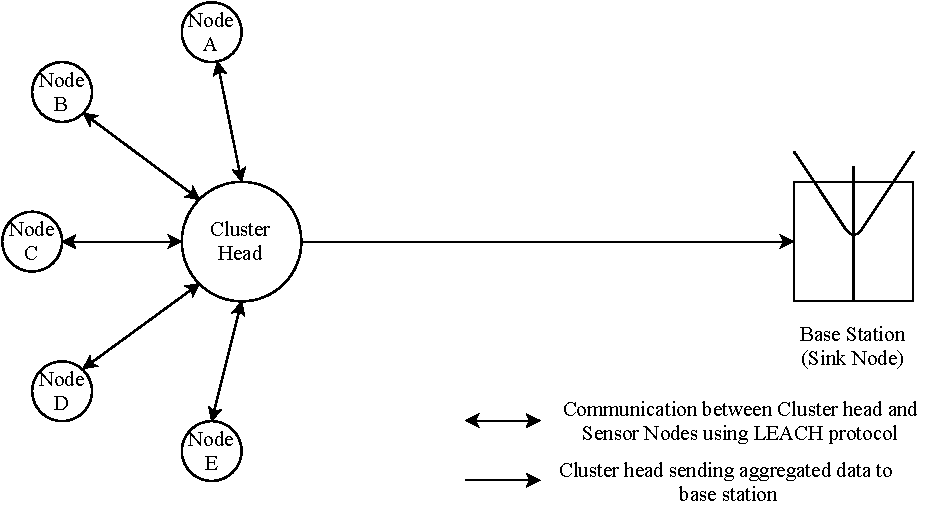
\includegraphics[scale=0.9]{Figures/PDF/SystemModel.pdf}
    \caption{System Model for dataset.}
    \label{SystemModel}	
    \end{figure}
This section presents the system model which is used in dataset. It is basically a model of LEACH-clustering routing algorithm. Figure \ref{SystemModel} describes how data from each sensor node is sent to cluster head. Cluster head processes data and after performing data aggregation it further sends it to base station.
%%%%%%%%%%%%%%%%%%%%%%%%%%%%%%%%%%%%%%%%%%%%%%%%%%%%%%%%%%%%%%%%%%%%%%%%%%%%%%%%%%%%%%%%%%%%%%%%%%%%%%%%%%%%%%%%%%%%%%%%%%%%%%%%%%%%%%%%
\section{Dataset} \label{S5.3}
WSN-DS\cite{almomani2016wsn} dataset used in this approach helps in classification and detection of attack. This dataset consists of LEACH-clustering protocol normal activities with attacks of like blackhole, grayhole, scheduling, and flooding. These attacks are implemented on top of LEACH protocol.
\par
To build the dataset it was required that each sensor node must monitor it's neighbor. Distribution of load and number of neighbor sensor nodes to monitor was a challenge which was taken care by many experiments. In the beginning of data collection, each node broadcasts \textit{Hello} message. After it, each node starts monitoring some nodes (5 nodes - result from experiments) from which it has received broadcast message. Then each node sends all details to it's cluster head which is further sent to base station at the end of each round. Dataset built with this procedure has 19 features which can help to know maliciousness of a node. These attributes are shown in table \ref{tab:WSNDS}.
\begin{longtable}[c]{|p{0.5in}|p{1.5in}|p{3.5in}|}
\caption{WSN-DS Description}
\label{tab:WSNDS}\\
\hline
\multicolumn{1}{|c|}{\textbf{S.N.}} & \multicolumn{1}{c|}{\textbf{Attribute}} & \multicolumn{1}{c|}{\textbf{Detail}} \\ \hline
\endfirsthead
%
\endhead
%
1. & Node ID & A unique ID for every node. E.g. 002 001 042 presents node number 42 in first round and second stage \\ \hline
2. & Time & Current time \\ \hline
3. & Is\_CH & Node is cluster head? (Flag - 0 or 1) \\ \hline
4. & who\_CH & Cluster head ID \\ \hline
5. & Dist\_to\_CH & distance b/w node and cluster head \\ \hline
6. & ADV\_S & no. of advertisement message broadcast to nodes by cluster head \\ \hline
7. & ADV\_R & no. of advertisement message received by nodes from cluster head \\ \hline
8. & JOIN\_S & no. of join request message sent to cluster head by nodes \\ \hline
9. & JOIN\_R & no. of join request message received by cluster head from nodes \\ \hline
10. & SCH\_S & no. of TDMA schedule message sent to nodes by cluster head \\ \hline
11. & SCH\_R & no. of TDMA schedule message received by nodes from cluster head \\ \hline
12. & Rank & node ordering in TDMA schedule message \\ \hline
13. & DATA\_S & no. of data packets sent to cluster head from sensor node \\ \hline
14. & DATA\_R & no. of data packets received by cluster head from sensor node \\ \hline
15. & Data\_Sent\_To\_BS & no. of data packets sent to base station by cluster head \\ \hline
16. & dist\_CH\_To\_BS & distance b/w cluster head and base station \\ \hline
17. & send\_code & cluster sending code \\ \hline
18. & Consumed energy & energy consumed \\ \hline
19. & Attack Type & Type of sensor node - blackhole, grayhole, scheduling, flooding or normal \\ \hline
\end{longtable}


\section{Proposed approach} \label{SPA}
This section describes how proposed system works. Basically, to simulate the attack environment, energy model of leach is implemented with attacks of like blackhole attack on top of leach which is described in section \ref{SSLeach}. Also, by using this WSN-DS dataset an Neural Network classifier is also trained to classify attack models which is presented in section \ref{SSNN}. Cumulatively, this approach can be referred as signature-based (rule-based or misuse) IDS. 
    \subsection{LEACH} \label{SSLeach}
    Wireless sensor network has some limitations described in section \ref{WSNChallenges}, like limited battery power. So, energy needs to be utilized efficiently in multihop wireless communication to minimize dead nodes, while network remains operational. To maintain continuous network services chosen communication protocol has to be energy efficient. The dataset WSN-DS was also created using such protocol – Low Energy Adaptive Clustering Hierarchy (LEACH). 
    \par LEACH \cite{palan2017low} is adaptive protocol which uses clustering of sensor node and distributes energy load equally in in all nodes of cluster. This routing algorithm works in two phases as shown in figure \ref{LeachPhases}. Phase 1 is Setup-phase where election of Cluster head, joining of member node in clusters, and TDMA time slots allotted to each member node by cluster head. In phase 2 which is steady-state phase, member nodes sends their data to cluster head in their allotted time slot. LEACH also involves data aggregation at cluster head, aggregated data is then sent to base station.
    \begin{figure}[h]
    \center	
    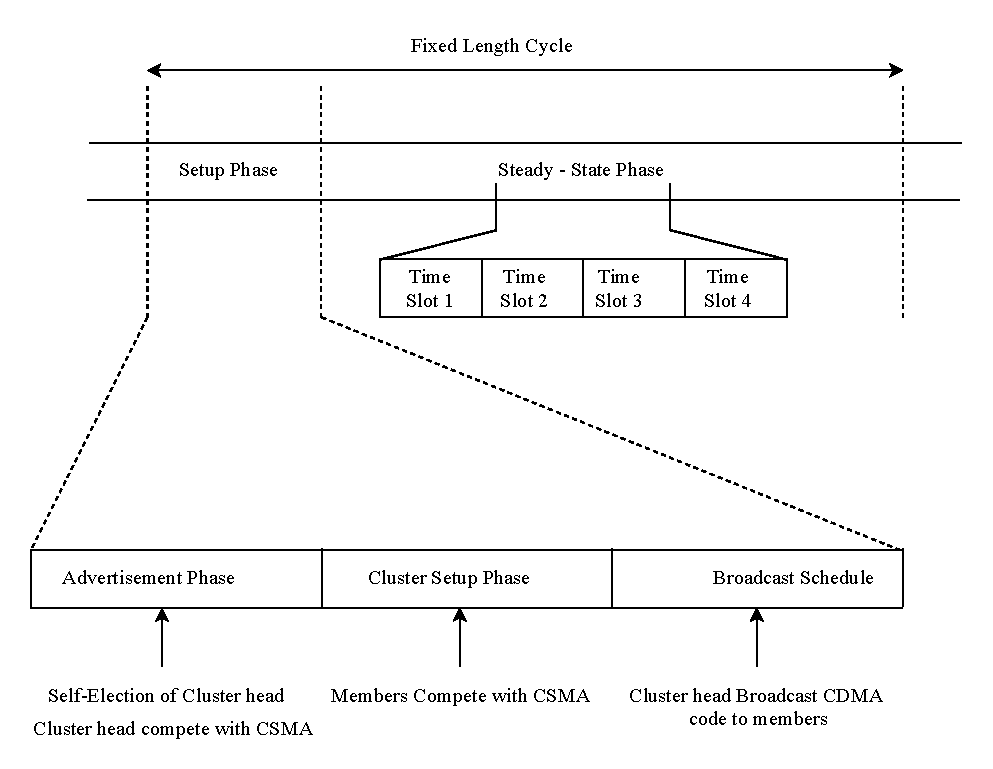
\includegraphics[scale=0.8]{Figures/PDF/LeachPhases.pdf}
    \caption{LEACH-Phases.}
    \label{LeachPhases}	
    \end{figure}
    \\
    \subsection{Neural Network} \label{SSNN}
    A neural network classifier consists of number of neurons units, arranged in layers. Each layer takes some input vector and gives output by applying a non-linear function. This output works as input to next layer in feed-forward manner. In general, there is no feedback to previous layer. Final output layer has implementation of classification of attack. Figure \ref{NN} shows Neural Network model of this proposed system.
    \begin{figure}[h]
    \center	
    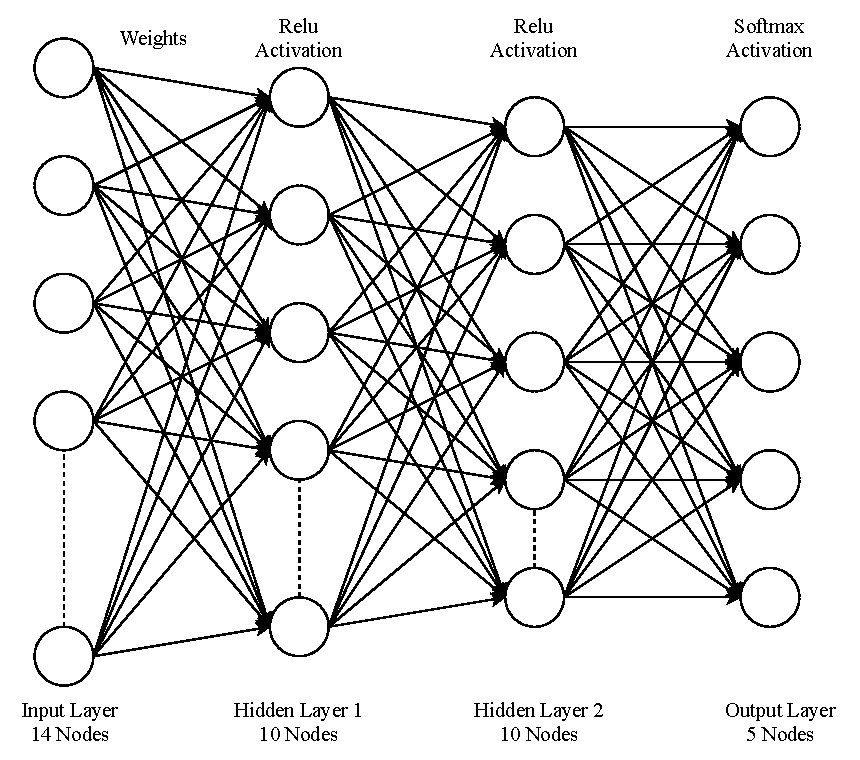
\includegraphics[scale=0.9]{Figures/PDF/NN.pdf}	
    \caption{Neural Network Model.}
    \label{NN}	
    \end{figure}
    
    \par In this work, we have used WSN-DS dataset to train our neural network which contains 374661 observations on different attacks on top of LEACH. The dataset contains data about Grayhole attack, Blackhole attack, Scheduling attack, Flooding attack together with normal behaviour of network in LEACH protocol. The dataset contains 19 features explained earlier in table \ref{tab:WSNDS}.
    \subsection{Flowchart}
    The process that is being used in this work to train network is learning process. Figure \ref{FlowChart} shows self-explanatory flowchart for learning process of neural network model.
        \begin{figure}[hbp]
        \center	
        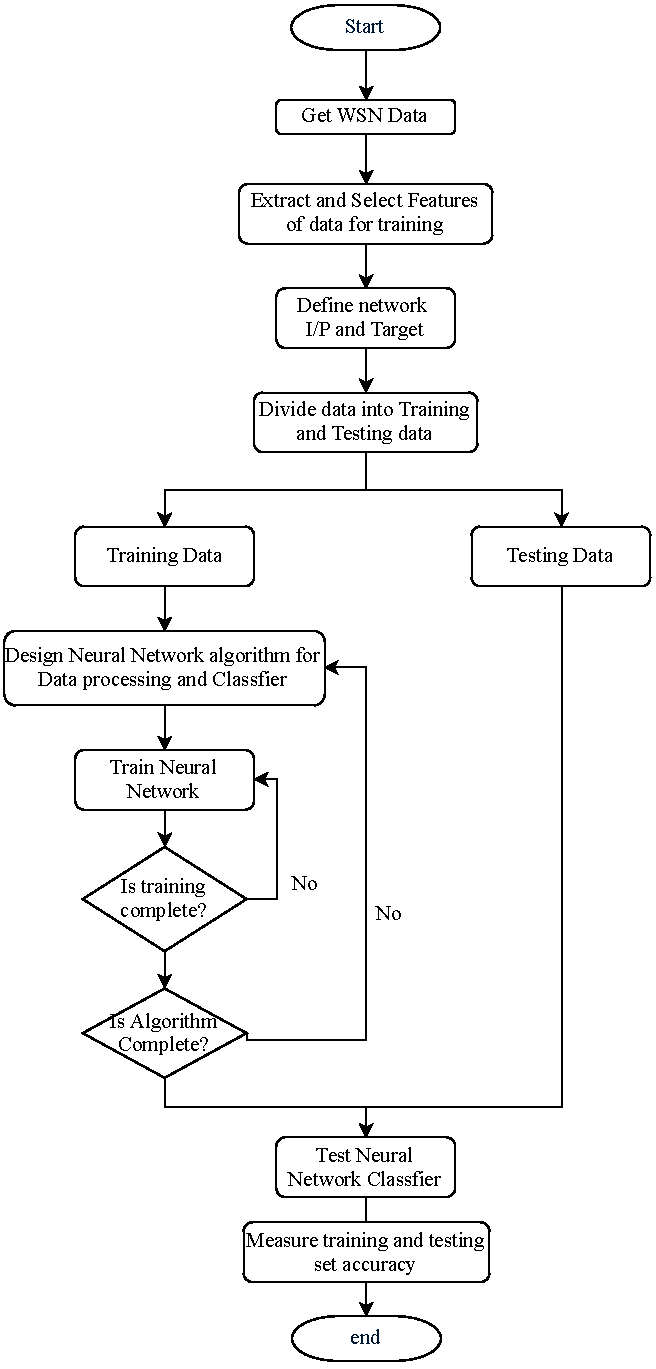
\includegraphics[width=4in, height=7.2in] {Figures/PDF/FlowChart.pdf}
        \caption{Flow Chart for Neural Network model}
        \label{FlowChart}	
        \end{figure}

\section{Procedure} \label{Procedure}
 To train this Neural Network one feature ‘Attack Type’ is used as label. Out of other remaining 18 features we have used 14 features to get the best result out of training. Training starts by building a sequential model using Keras API which is a high-level API to build and train models in Tensorflow (an online machine learning library for research) . This sequential model assemble layers in stack. This model has a flexibility to add number of hidden layers using its built in functions. Detailed working of neural network model is explained in this section.
Neural Network working model can be described in following 6 steps:
\begin{enumerate}[label=\textbf{\roman*}]
\item \textbf{Analyze the Dataset } Data is very important in every application of Neural Network learning. Analyzing data helps in feature extraction and selection. Analyzing dataset also includes analyzing Dataset, Attribute characteristics, Number of Instances, Attributes etc. Here, data is analyzed with the help of Pandas library of python. 
\item \textbf{Prepare the dataset } Raw data is of no use. To make use of any data it must be structured in proper way. Here, representation of analyzed data in a n-dimensional matrix is done using NumPy library of python.

\item \textbf{Create the Model } Neural networks large number of neurons are arranged in sequential layer using 'Sequential' model of Keras API. Here, neural network fully connected layered model was created using 'Dense' function. Our model has 1 I/P, 2 hidden, 1 O/P classification layers as shown in figure \ref{NN}. I/P layer was initialized with 14 neurons (14 selected features). Relu (Rectified linear unit) activation function was used for I/P, and hidden layer with uniform weight distribution. Softmax activation function was used for O/P classification layer.

\item \textbf{Compile the Model } To compile this model 'loss', 'optimizer', and 'metrics' parameters are needed to make neural network learn during each iteration. We have used 'categorical\_crossentropy' is loss function to minimize the error term between expected and actual output. 'Adam' optimizer is used to search for different weights for neuron connections. We have used 'accuracy' as metrics to measure the classification accuracy. 

\item \textbf{Fit the Model } Compiled model is ready to be trained using dataset. To fit data into model keras gives 'fit' function which accepts training I/P data, training O/P data, validation data, iterations.

\item \textbf{Evaluate the Model } After fitting data into model its evaluation is required. 'Evaluation' function of model takes input data and actual output data. It predicts output using input data based on what it has learned, which is then compared with actual output. 

\end{enumerate}    

        
% \section{Experimental results} \label{S5.4}
% In this section, the performance of anisotropic shaped region ..........................
% \subsection{Choice of parameters in the proposed approach} \label{SS5.4.1}
% For all experiments, the size of region and subregion 
\section{Summary} \label{SSummary}
In this chapter, a supervised Neural network learning approach has been discussed which helps to build signature-based IDS using dataset. The proposed algorithm can be divided into two parts. In first part data collection, data analysis, and data preparation is done. Dataset is divided into 75-25\% as training and testing data.  Training data is then fed into neural network model for training purpose. After completion of training model evaluation is performed using testing dataset. Evaluation results have been shown in section \ref{NNresults}.
After that in second part, to simulate the WSN environment (mainly LEACH protocol and attacks), energy model of WSN is implemented in Octave. Evaluation of this part is done by analyzing energy left in the network, dead and alive nodes, data packets delivered to CH and BS etc. Evaluation results of this part is shown in chapter \ref{C6}.
%\clearpage
%%%%%%%%%%%%%%%%%%%%%%%%%%%%%%%%%%%%%%%%%%%%%%%%%%%%%%%%%%%%%%%%%%%%%%%%%%%%%%%%%
 